\documentclass[twocolumn, 10pt, a4paper]{article}
\usepackage[a4paper, left = 0.5cm,right = 0.5cm, top = 0.5cm, bottom = 1cm, footskip = 0.5cm]{geometry}
\usepackage{amsmath}
\usepackage{graphicx}
\usepackage{subfig}
\usepackage{float}
\usepackage{wrapfig}
\usepackage{lipsum}
\usepackage{tikz}
\usepackage{arydshln}
\usepackage{pgfplots}
\usepackage[style = numeric, sorting = none]{biblatex}
 
\addbibresource{refs.bib}

\graphicspath{{./images/}}

\usetikzlibrary{shapes.geometric, arrows, calc}
\tikzstyle{startstop} = [rectangle, rounded corners, minimum width=0cm, minimum height=0cm, text centered, text width=1cm, draw=black, fill=white!30]
\tikzstyle{process} = [rectangle, minimum width=0cm, minimum height=0cm, text centered, text width=4.8cm, draw=black, fill=white!30]
\tikzstyle{decision} = [diamond, aspect = 1.25, minimum width=0cm, minimum height=0cm, text centered, text width=3cm, draw=black, fill=white!30, inner sep = -1.5ex]
\tikzstyle{arrow} = [thick,->,>=stealth]

\pgfplotsset{compat = 1.17}

\author{
  % George Herbert\\
  % \texttt{cj19328@bristol.ac.uk}
}
\date{}

\title{\vspace{-2em}No Entry Sign Challenge Report\vspace{-2em}}

\begin{document}

\maketitle

\section{The Viola-Jones object detector}

\subsection{Ground truth and visualisation}

\begin{figure}[htbp]
  \centering
  \subfloat[\texttt{NoEntry1.jpg}]{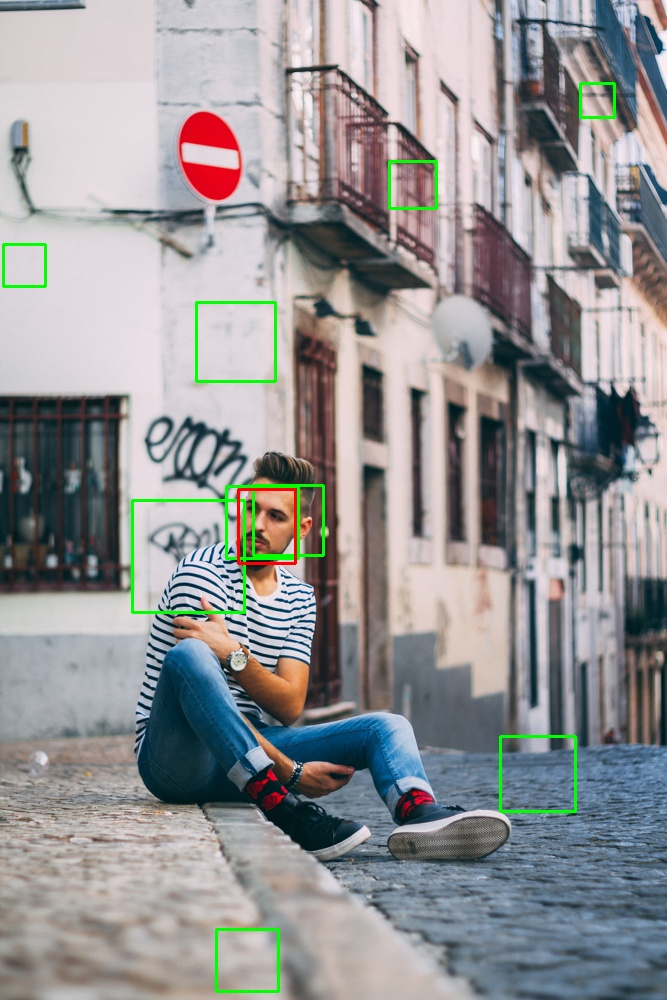
\includegraphics[width = 0.24\textwidth]{images/NoEntry1.jpg}\label{fig:face1}}
  \hfill
  \subfloat[\texttt{NoEntry2.jpg}]{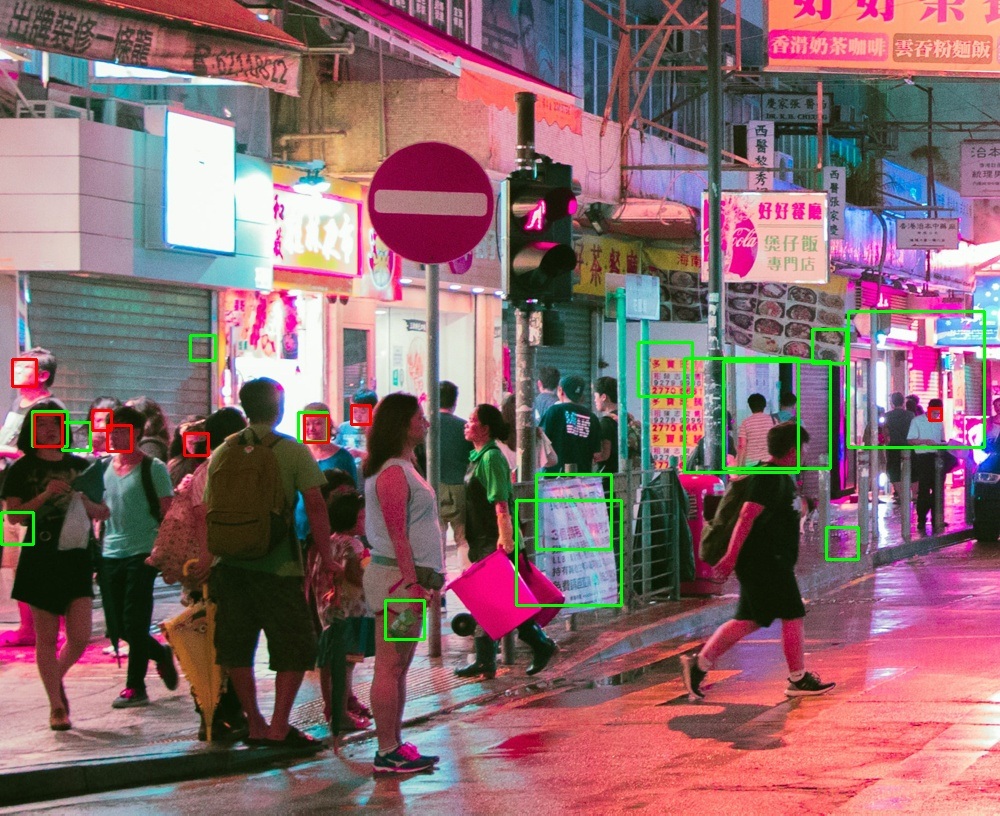
\includegraphics[width = 0.24\textwidth]{images/NoEntry2.jpg}\label{fig:face2}}
  \hfill
  \subfloat[\texttt{NoEntry4.jpg}]{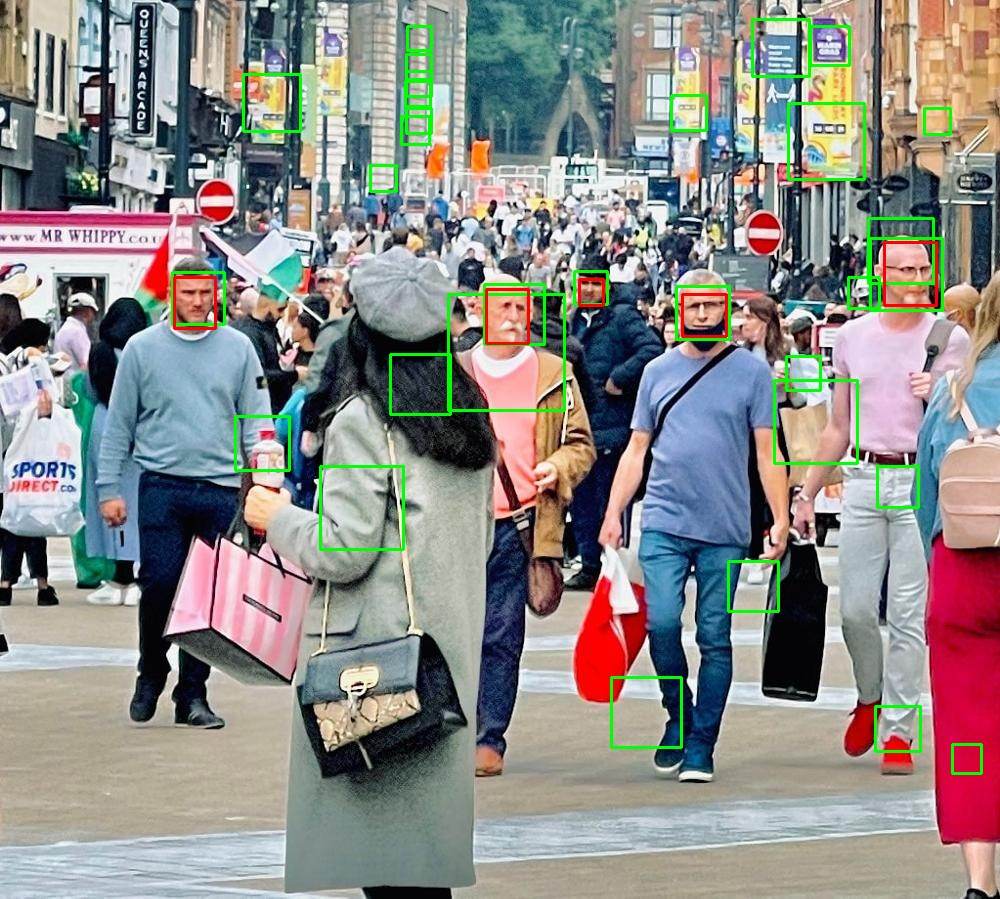
\includegraphics[width = 0.24\textwidth]{images/NoEntry4.jpg}\label{fig:face4}}
  \hfill
  \subfloat[\texttt{NoEntry5.jpg}]{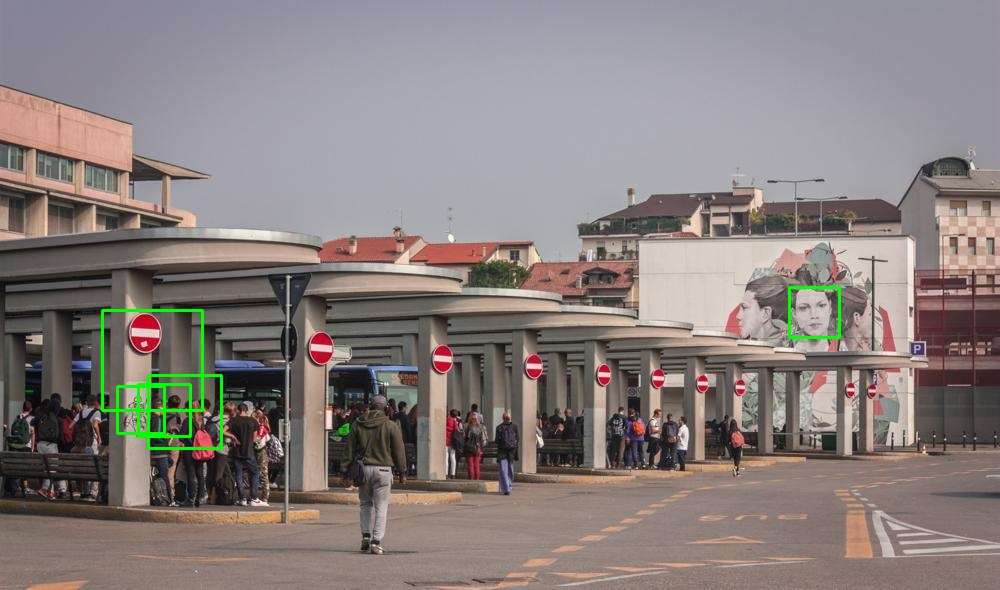
\includegraphics[width = 0.24\textwidth]{images/NoEntry5.jpg}\label{fig:face5}}
  \hfill
  \subfloat[\texttt{NoEntry7.jpg}]{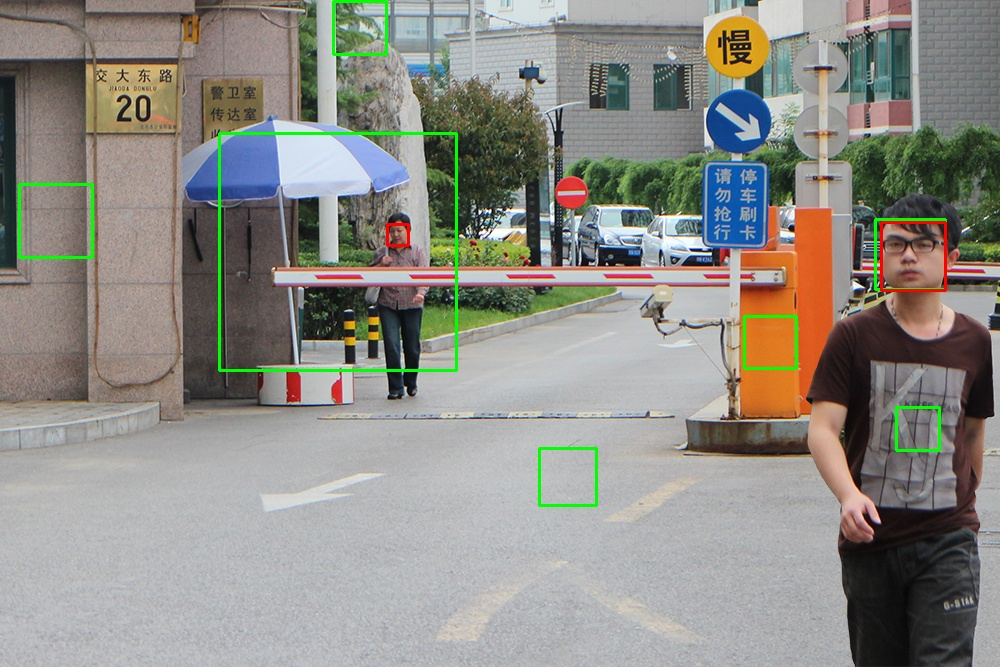
\includegraphics[width = 0.24\textwidth]{images/NoEntry7.jpg}\label{fig:face7}}
  \hfill
  \subfloat[\texttt{NoEntry11.jpg}]{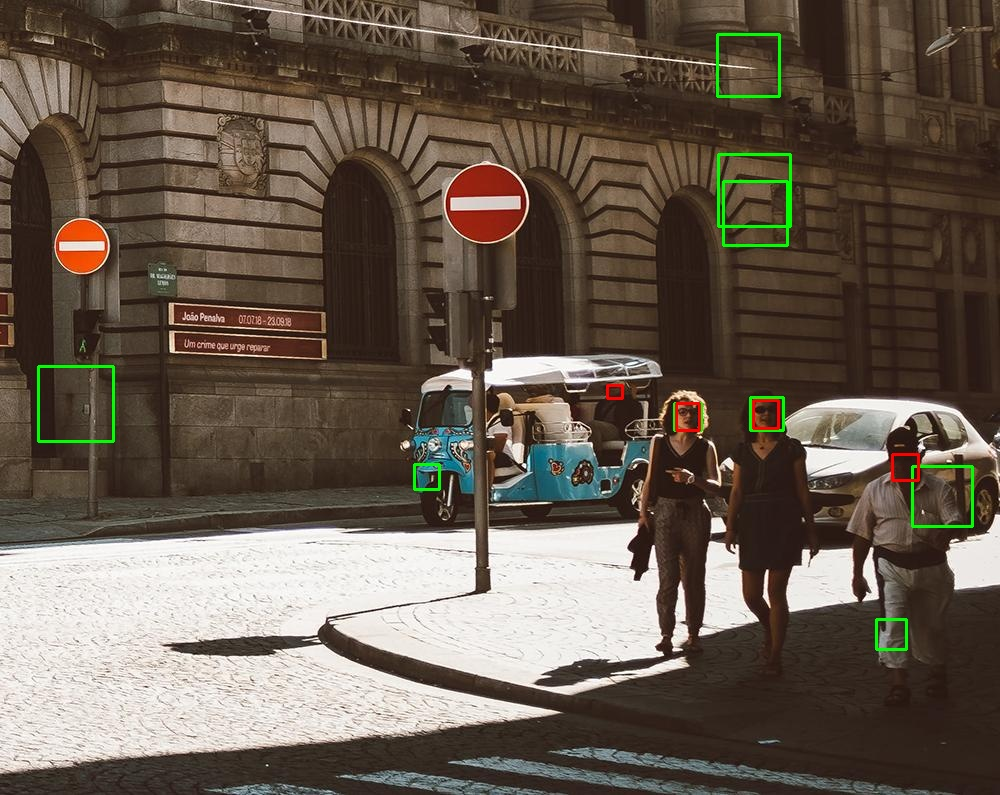
\includegraphics[width = 0.24\textwidth]{images/NoEntry11.jpg}\label{fig:face11}}
  \caption{Six images with the ground truth bounding boxes in red and actually detected instances from \texttt{face.cpp} in green}\label{fig:face}
\end{figure}

Ground truth bounding boxes assist in determining the accuracy of a detection algorithm, and help to visualise how well it performs.
Figure \ref{fig:face} displays six images, with their ground truth bounding boxes in red, and the frontal faces detected by \texttt{face.cpp} in green.
I defined the ground truth frontal faces as those whereby the majority of the face was visible, the person was facing the camera (i.e. both eyes visible) and the person was close enough for the major facial characteristics distinguishable.

\subsection{Intersection-over-union, true positve rate and F\textsubscript{1} score}

True positive rate (TPR) is a popular metric used to assess the performance of an object detection algorithm.
The TPR is the proportion of objects that an algorithm is attempting to detect that are actually detected, and is given by the formula:
\[
  \textrm{TPR} = \frac{\textrm{TP}}{\textrm{TP + FN}}
\]
where TP is the number of true positives, and FN is the number of false negatives.

The first practical difficulty that arises in calculating the TPR is whether or not to define a predicted bounding box as a being a true positive or a false positive.
I opted to define a detected bounding box as being a true positive if it had an intersection-over-union (IOU) value greater than 0.5 with a ground truth bounding box, as this is considered a good score \cite{iou}.
For two bounding boxes $A$ and $B$, the IOU is calculated as follows:
\[
  \textrm{IOU}(A, B) = \frac{|A \cap B|}{|A \cup B|}
\]
where $|A \cap B|$ is the area of intersection, and $|A \cup B|$ is the area of union.
Moreover, for each ground truth bounding box, I only defined the detected bounding box with the largest IOU value as being a true positive if there was more than one intersecting detected bounding box.

In any detection task, TPR can be a flawed metric to use to define how well a given model performs.
This is because, firstly, the TPR can be usually be artificially increased simply by lowering the IOU threshold, without the model actually performing any better in reality.
Secondly, it is possible to achieve a TPR of 100\% by detecting every possible pixel region as being the object being detected, despite having a large number of false positives.

As a result of this, the F\textsubscript{1} score is often used as a measure of a model's accuracy.
F\textsubscript{1} score is the harmonic mean of recall (i.e. TPR) and precision (i.e. the proportion of predicted positives that are actually positive), and is calculated as follows:
\[
  \textrm{F\textsubscript{1}} = \frac{\textrm{TP}}{\textrm{TP} + \frac{1}{2}(\textrm{FP} + \textrm{FN})}
\]
where FP is the number of false positives. 

\begin{table}[htbp]
  \begin{center}
  \caption{TPRs and F\textsubscript{1} scores of the frontal face detector}\label{tab:face}
  \begin{tabular}{l | l l} 
    \hline\hline
    Image&TPR&F\textsubscript{1} Score\\
    \hline
    \texttt{NoEntry0.jpg}&Undefined&0.00\\ 
    \texttt{NoEntry1.jpg}&1.00&0.20\\ 
    \texttt{NoEntry2.jpg}&0.25&0.18\\ 
    \texttt{NoEntry3.jpg}&Undefined&Undefined\\ 
    \texttt{NoEntry4.jpg}&1.00&0.28\\ 
    \texttt{NoEntry5.jpg}&Undefined&0.00\\ 
    \texttt{NoEntry6.jpg}&Undefined&0.00\\ 
    \texttt{NoEntry7.jpg}&0.50&0.22\\ 
    \texttt{NoEntry8.jpg}&Undefined&0.00\\ 
    \texttt{NoEntry9.jpg}&Undefined&0.00\\ 
    \texttt{NoEntry10.jpg}&Undefined&0.00\\ 
    \texttt{NoEntry11.jpg}&0.50&0.31\\ 
    \texttt{NoEntry12.jpg}&0.00&0.00\\ 
    \texttt{NoEntry13.jpg}&Undefined&0.00\\ 
    \texttt{NoEntry14.jpg}&Undefined&0.00\\ 
    \texttt{NoEntry15.jpg}&Undefined&0.00\\ 
    \hdashline
    All images&0.52&0.15\\ 
    \hline
  \end{tabular}
  \end{center}
\end{table} 

Table \ref{tab:face} displays the TPR and F\textsubscript{1} score that \texttt{face.cpp} achieved on each of the \texttt{NoEntry\textasteriskcentered.jpg} images.
Due to the definitions of TPR and F\textsubscript{1} score, many of the values are undefined since division by zero yields an undefined result.

\clearpage

\section{Building and testing my own detector}

\subsection{Training performance}

\begin{figure}[h]
  \pgfplotstableread{
  0 1        1
  1 1        0.0214601
  2 1        0.000129286
  }\dataset
  \begin{tikzpicture}
  \begin{axis}[
    ybar,
    ymode = log,
    log origin = infty,
    width = 0.49\textwidth,
    ymax = 1,
    enlarge x limits = 0.25,
    enlarge y limits = 0.05,
    ylabel = {Rate},
    xlabel = {Training Stage},
    xtick = data,
    xticklabels = {0, 1, 2},
  ]
  \addplot[draw = black, fill = green!50] table[x index = 0,y index = 1] \dataset;
  \addplot[draw = black, fill = red!50] table[x index = 0,y index = 2] \dataset;
  \legend{TPR, FPR}
  \end{axis}
  \end{tikzpicture}
  \caption{TPR and FPR of stages in the Viola-Jones no entry sign training process}\label{vj_training}
\end{figure}

During the Viola-Jones no entry sign training process, the false positive rate (FPR) is the number of negatives incorrectly predicted as being a positive no entry sign.
Figure \ref{vj_training} displays the TPR and FPR at each stage of the training process.
At each successive stage, the TPR remains at 100\%, while the FPR decreases drastically.
 
\subsection{Testing performance}

\begin{figure}[htbp]
  \centering
  \subfloat[\texttt{NoEntry2.jpg}]{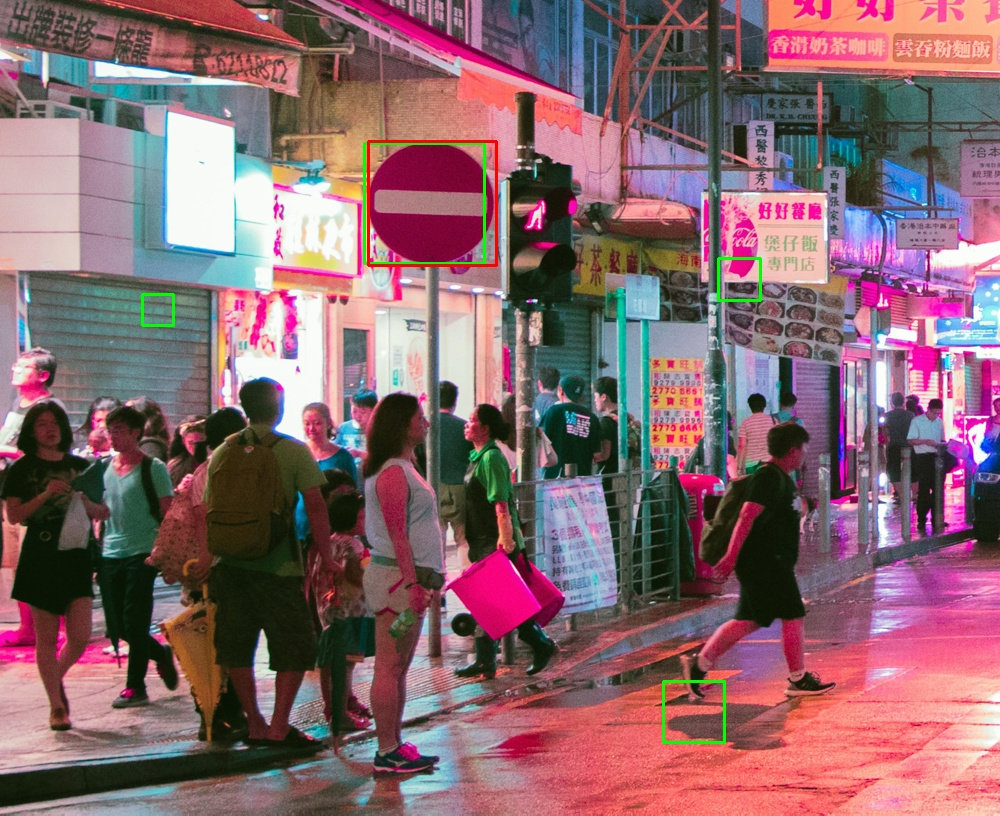
\includegraphics[width = 0.3115\textwidth]{images/task_2_2.jpg}\label{fig:task_2_2}}
  \hfill
  \subfloat[\texttt{NoEntry8.jpg}]{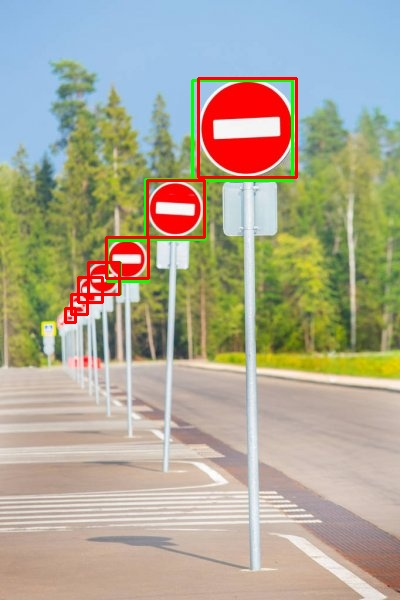
\includegraphics[width = 0.1695\textwidth]{images/task_2_8.jpg}\label{fig:task_2_8}}
  \hfill
  \subfloat[\texttt{NoEntry3.jpg}]{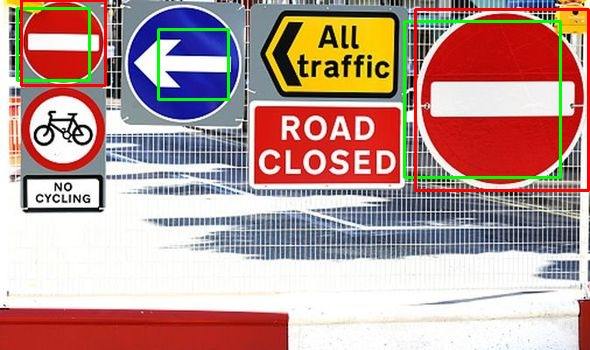
\includegraphics[width = 0.49\textwidth]{images/task_2_3.jpg}\label{fig:task_2_3}}
  \caption{Three images with the bounding boxes of the ground truths in red and actually detected instances in green from the Viola-Jones no entry sign detector}\label{fig:task_2}
\end{figure}

Figure \ref{fig:task_2} contains three images with ground truth bounding boxes in red, and detected bounding boxes from the Viola-Jones implementation in green.
The implementation works relatively well, achieving a TPR of 0.44 and an F\textsubscript{1} score of 0.48, as shown in Table \ref{tab:vj}.
However, the implementation has its shortcomings.
When tested, the Viola-Jones implementation detects a large number of false positives.
Upon inspection, this primarily occurs in regions containing a slightly lighter strip horizontally between two darker strips.
For example, the turn left sign in Figure \ref{fig:task_2_3} has been incorrectly detected in this manner.

The TPR on the test data is significantly lower than on the training data.
One reason for this is likely due to the differing appearances of no entry signs in the test data.
The Viola-Jones implementation was trained using a single no entry sign with different perspective transformations applied to it to create a collection of artificial positives.
This approach works best for completely rigid objects \cite{training}. 
However, due to the slightly differing appearances of the no entry signs between countries, the positives in our test images are not.
Additionally, we are only testing our implementation on 16 images.
To get a more accurate idea of the true TPR and F\textsubscript{1} score, we would need to test our implementation on a larger test set.

\begin{table}[htbp]
  \begin{center}
  \caption{TPRs and F\textsubscript{1} scores of Viola-Jones no entry sign detector}\label{tab:vj}
  \begin{tabular}{l | l l} 
    \hline\hline
    Image&TPR&F\textsubscript{1} Score\\
    \hline
    \texttt{NoEntry0.jpg}&1.00&0.67\\ 
    \texttt{NoEntry1.jpg}&1.00&0.40\\ 
    \texttt{NoEntry2.jpg}&1.00&0.40\\ 
    \texttt{NoEntry3.jpg}&1.00&0.80\\ 
    \texttt{NoEntry4.jpg}&0.50&0.67\\ 
    \texttt{NoEntry5.jpg}&0.40&0.47\\ 
    \texttt{NoEntry6.jpg}&0.00&0.00\\ 
    \texttt{NoEntry7.jpg}&0.00&0.00\\
    \texttt{NoEntry8.jpg}&0.57&0.72\\ 
    \texttt{NoEntry9.jpg}&0.00&0.00\\ 
    \texttt{NoEntry10.jpg}&0.67&0.67\\ 
    \texttt{NoEntry11.jpg}&0.50&0.25\\ 
    \texttt{NoEntry12.jpg}&0.25&0.40\\ 
    \texttt{NoEntry13.jpg}&0.00&0.00\\ 
    \texttt{NoEntry14.jpg}&1.00&1.00\\ 
    \texttt{NoEntry15.jpg}&0.50&0.67\\ 
    \hdashline
    All images&0.44&0.48\\ 
    \hline
  \end{tabular}
  \end{center}
\end{table} 

\clearpage

\section{Integration with shape detectors}

\subsection{Hough Details}

\begin{figure}[H]
  \vspace{-4.5em}
  \centering
  \subfloat[\texttt{NoEntry6.jpg} with detected bounding boxes]{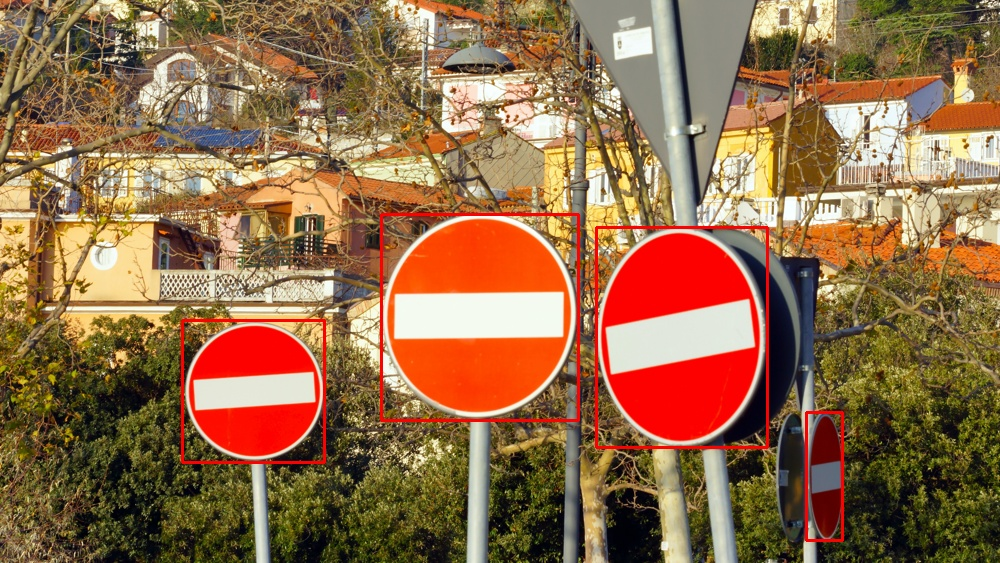
\includegraphics[width = 0.24\textwidth]{images/task_3_6.jpg}}
  \hfill
  \subfloat[\texttt{NoEntry2.jpg} with detected bounding boxes]{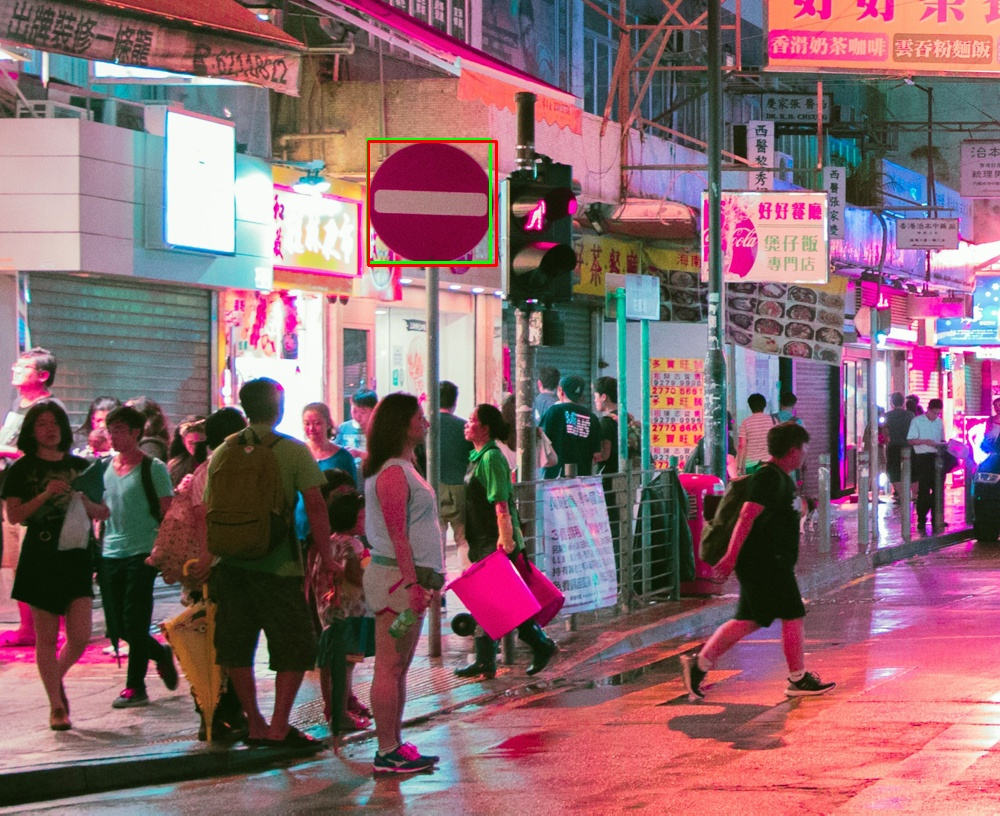
\includegraphics[width = 0.24\textwidth]{images/task_3_2.jpg}}
  \hfill
  \subfloat[\texttt{NoEntry6.jpg} gradient magnitude threshold]{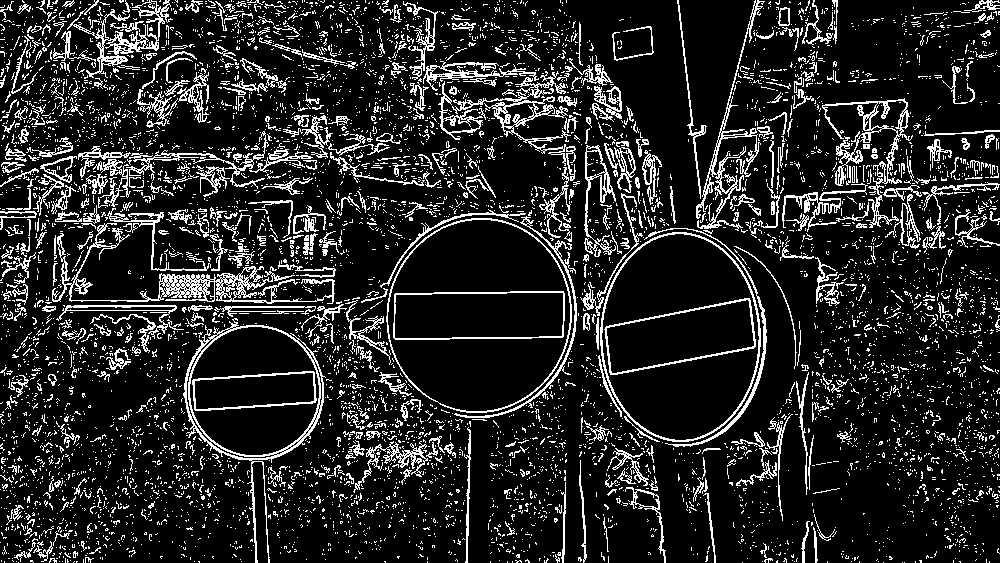
\includegraphics[width = 0.24\textwidth]{images/6_gradient_magnitude_threshold.jpg}}
  \hfill
  \subfloat[\texttt{NoEntry2.jpg} gradient magnitude threshold]{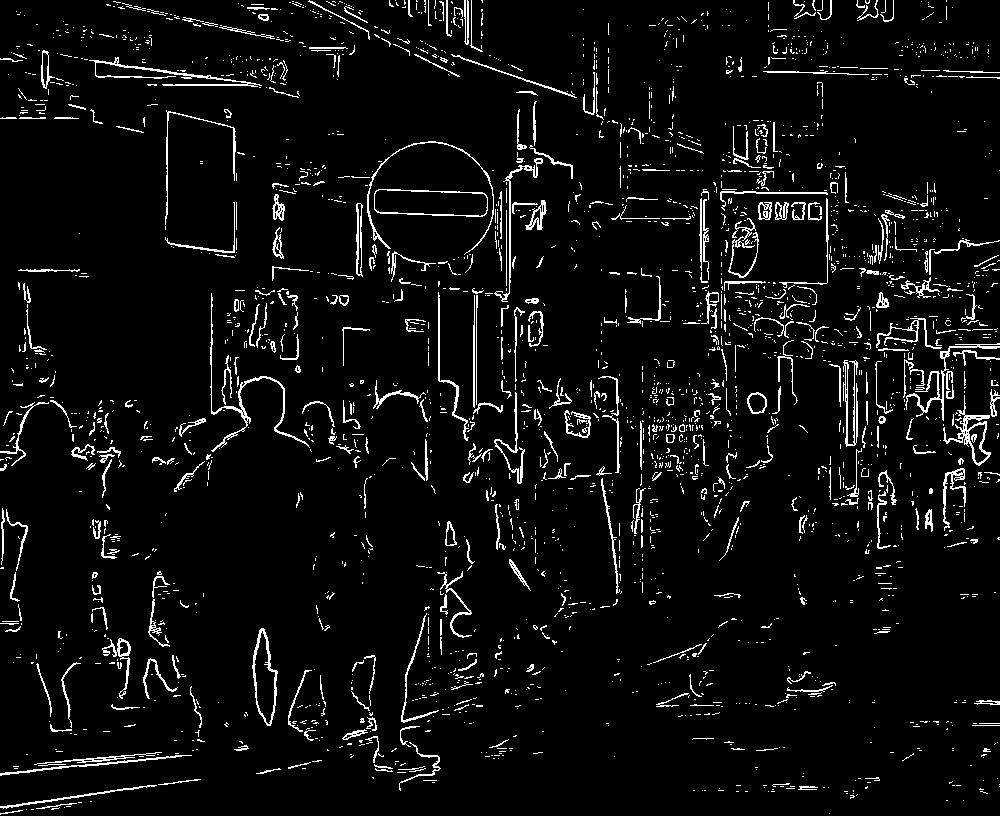
\includegraphics[width = 0.24\textwidth]{images/2_gradient_magnitude_threshold.jpg}}
  \hfill
  \subfloat[\texttt{NoEntry6.jpg} 2D Hough space]{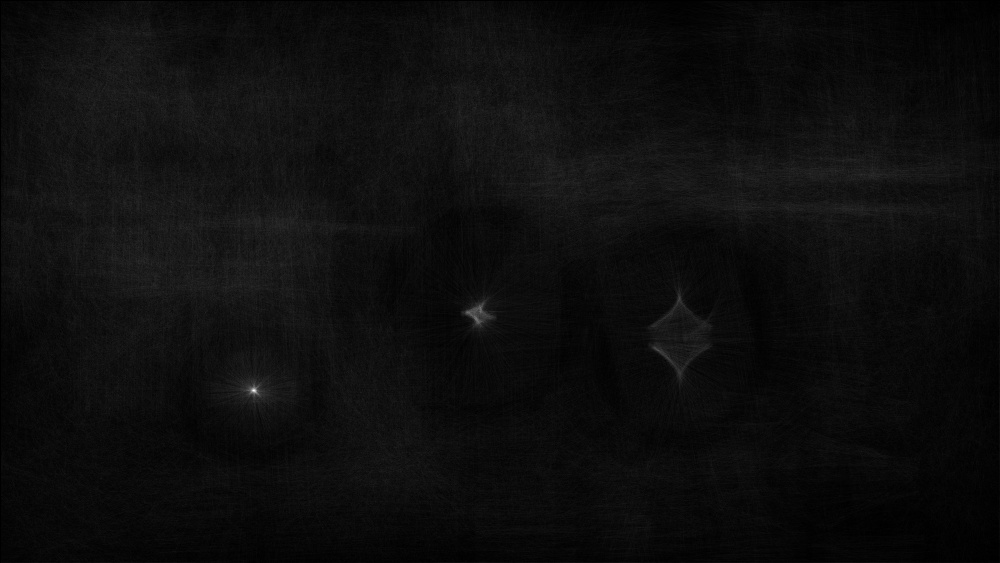
\includegraphics[width = 0.24\textwidth]{images/6_hough_space.jpg}}
  \hfill
  \subfloat[\texttt{NoEntry2.jpg} 2D Hough space]{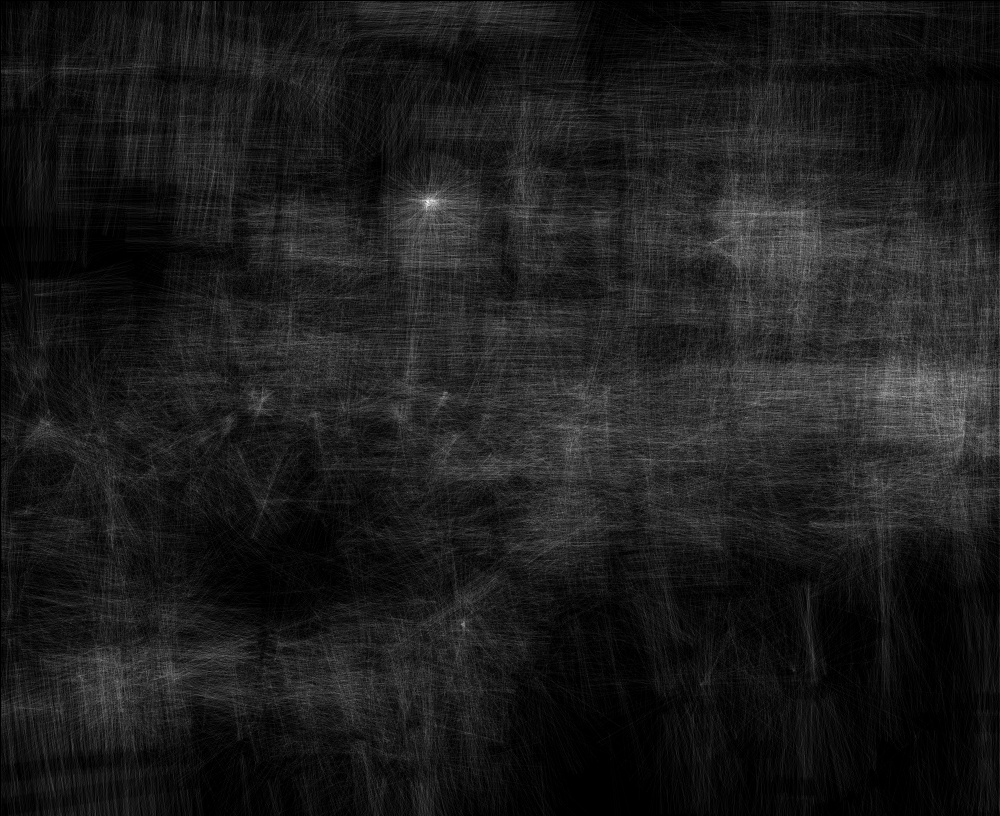
\includegraphics[width = 0.24\textwidth]{images/2_hough_space.jpg}}
  \caption{Two no entry sign images at various stages of the integrated implementation}\label{fig:hough_details}
\end{figure}

\subsection{Evaluation}

Table \ref{tab:shape} displays the TPR and F\textsubscript{1} score of the integrated implementation, as well as the differences compared with the Viola-Jones implementation.
The key merits and shortcomings include:
\begin{itemize}
\itemsep 0em 
\item A significantly larger F\textsubscript{1} score, primarily as a result of increasing the precision; achieved by only defining an object detected by the Viola-Jones detector as positive if it has an IOU value with a  bounding box from the circle Hough transform greater than 50\%
\item A small improvement to the TPR score, by reducing the minimum  number of neighbours allowing for more true positives to be identified (the extra false positives were `filtered out' by utilising the circle Hough transform)
\item If a no entry sign is positively detected by one of the detectors, but not the other, it is not positively detected by the integrated implementation
\item A significantly slower implementation, since the circle Hough transform takes longer to calculate
\end{itemize}

\subsection{Detection pipeline}

Figure \ref{fig:flow} outlines the way I combined evidence in my algorithm.
The rationale behind this was as follows:
\begin{itemize}
\itemsep 0em 
\item The Viola-Jones detector detected 44\% of no entry signs, but had a low level of precision
\item Upon inspection of the detected bounding boxes, it became clear the Viola-Jones detector appeared to be detecting regions with a light bar horizontally between two dark bars
\item Since no entry signs are circles, we could choose to detect the circles from the circle Hough transform that have an IOU with a Viola-Jones bounding box of greater than 50\% (i.e. they are likely detecting the same object)
\end{itemize}

\begin{table}[H]
  \begin{center}
  \caption{TPRs and F\textsubscript{1} scores of the integrated implementation, and the differences compared to the Viola-Jones implementation}\label{tab:shape}
  \begin{tabular}{l | l l | l l} 
    \hline\hline
    &\multicolumn{2}{| c |}{Result}&\multicolumn{2}{| c}{Difference}\\
    Image&TPR&F\textsubscript{1} Score&TPR&F\textsubscript{1} Score\\
    \hline
    \texttt{NoEntry0.jpg}&1.00&1.00&$\pm0.00$&+0.33\\
    \texttt{NoEntry1.jpg}&1.00&1.00&$\pm0.00$&+0.60\\
    \texttt{NoEntry2.jpg}&1.00&1.00&$\pm0.00$&+0.60\\
    \texttt{NoEntry3.jpg}&1.00&1.00&$\pm0.00$&+0.20\\
    \texttt{NoEntry4.jpg}&1.00&1.00&+0.50&+0.33\\
    \texttt{NoEntry5.jpg}&0.20&0.31&$-0.20$&$-0.16$\\
    \texttt{NoEntry6.jpg}&0.00&0.00&$\pm0.00$&$\pm0.00$\\
    \texttt{NoEntry7.jpg}&0.00&0.00&$\pm0.00$&$\pm0.00$\\
    \texttt{NoEntry8.jpg}&0.43&0.60&$-0.14$&$-0.13$\\
    \texttt{NoEntry9.jpg}&1.00&1.00&+1.00&+1.00\\
    \texttt{NoEntry10.jpg}&1.00&1.00&+0.33&+0.33\\
    \texttt{NoEntry11.jpg}&0.50&0.67&$\pm0.00$&+0.42\\
    \texttt{NoEntry12.jpg}&0.38&0.55&+0.13&+0.16\\
    \texttt{NoEntry13.jpg}&0.00&0.00&$\pm0.00$&$\pm0.00$\\
    \texttt{NoEntry14.jpg}&1.00&1.00&$\pm0.00$&$\pm0.00$\\
    \texttt{NoEntry15.jpg}&1.00&1.00&+0.50&+0.33\\
    \hdashline
    All images&0.50&0.66&+0.04&+0.17\\
    \hline
  \end{tabular}
  \end{center}
\end{table} 

\begin{figure}[H]
\centering
\resizebox{0.45\textwidth}{!}{
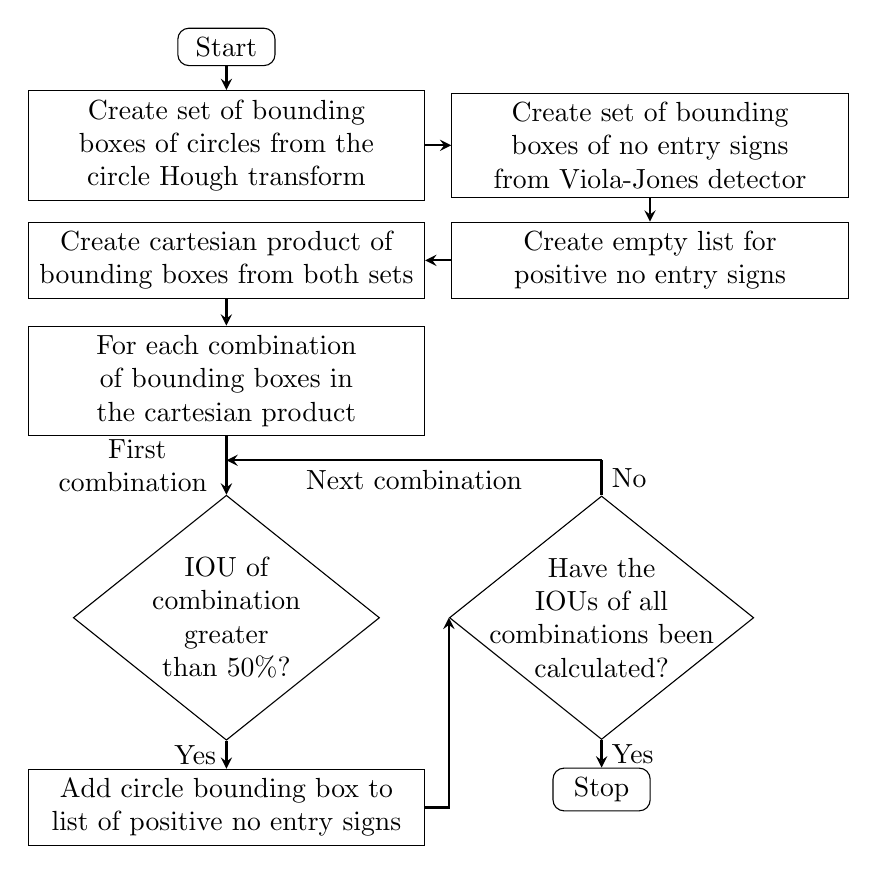
\begin{tikzpicture}[node distance = 1.25cm]
  \node (start) [startstop] {Start};
  \node (hough) [process, below of = start] {Create set of bounding boxes of circles from the circle Hough transform};
  \node (vj) [process, right of = hough, xshift = 11.75em] {Create set of bounding boxes of no entry signs from Viola-Jones detector};
  \node (empty) [process, below of = vj, yshift = -0.6em] {Create empty list for positive no entry signs};
  \node (cartesian) [process, left of = empty, xshift = -11.75em] {Create cartesian product of bounding boxes from both sets};
  \node (for) [process, below of = cartesian, yshift = -0.8em] {For each combination of bounding boxes in the cartesian product};
  \node (iou) [decision, below of = for, yshift = -5em] {IOU of\\combination greater\\than 50\%?};
  \node (list) [process, below of = iou, yshift = -3.3em] {Add circle bounding box to list of positive no entry signs};
  \node (done) [decision, right of = iou, xshift = 10em] {Have the\\IOUs of all\\combinations been\\calculated?};
  \node (stop) [startstop, below of = done, yshift = -2.65em] {Stop};
  \draw [arrow] (start) -- (hough);
  \draw [arrow] (hough) -- (vj);
  \draw [arrow] (vj) -- (empty);
  \draw [arrow] (empty) -- (cartesian);
  \draw [arrow] (cartesian) -- (for);
  \draw [arrow] (for) -- node[anchor = east, text width = 2cm] {\centering First\\combination} (iou);
  \draw [arrow] (iou) -- node[anchor = east] {Yes} (list);
  \draw [arrow] (list.east) -| (done.west);
  \draw let \p1 = (done.north) in [thick,-] (done.north) -- node[anchor = west] {No} (\x1, -5.25);
  \draw let \p1 = (done.north), \p2 = (iou.north) in [arrow] (\x1, -5.25) -- node[anchor = north] {Next combination} (\x2, -5.25);
  \draw [arrow] (done) -- node[anchor = west] {Yes} (stop);
\end{tikzpicture}
}
\caption{Flow chart detailing my algorithm that integrates Viola-Jones with the circle Hough transform}
\label{fig:flow}
\end{figure}

\clearpage

\section{Improving my detector}

\subsection{Idea}

The motivation behind the new approach came from identifying the areas whereby the previous approach failed.
There were several no entry signs that were visually quite clear (i.e. big, no occlusion, etc.), and were identified by the circle Hough transform, but since the Viola-Jones detector did not identify them, they were not positively identified.
Therefore, to improve the detector, I took every circle rejected by the previous approach, and put them through an extra stage of processing.

The extra stage of processing worked on the principal that every no entry sign shares similar characteristics.
They contain two colours: red and white; and they have a horizontal bar in the middle.
To identify the main colours in each circle, my algorithm first transforms the colour space of the pixels within the circle from RGB to CIELAB.
Since CIELAB uses perceptual brightness $L*$ as one of the values, my algoritm ignores this field and instead focus on the green-red axis $a*$ and the blue-yellow axis $b*$.
This is an advantage since it enables my algorithm to identify the colours in the no entry signs, despite the lighting levels.
My algorithm then performs $k$-means clustering on the $a*$ and $b*$ axes, to identify the two primary colours in each circle.
Since CIELAB is designed to be perceptually uniform, my algorithm then calculates the Euclidean distance from pure white and pure red to the two cluster centers, to identify whether the primary colours in the circle were red and white.
If the two primary colours are red and white, and there is more red in the circle than white, my algorithm then performs the line Hough transform on the circle.
If the circle contains two approximately horizontal parallel lines, the circle is accepted as another positive no entry sign.

\subsection{Visualise}

\begin{figure}[H]
  \vspace{-4.5em}
  \centering
  \subfloat[\texttt{NoEntry6.jpg} with detected bounding boxes]{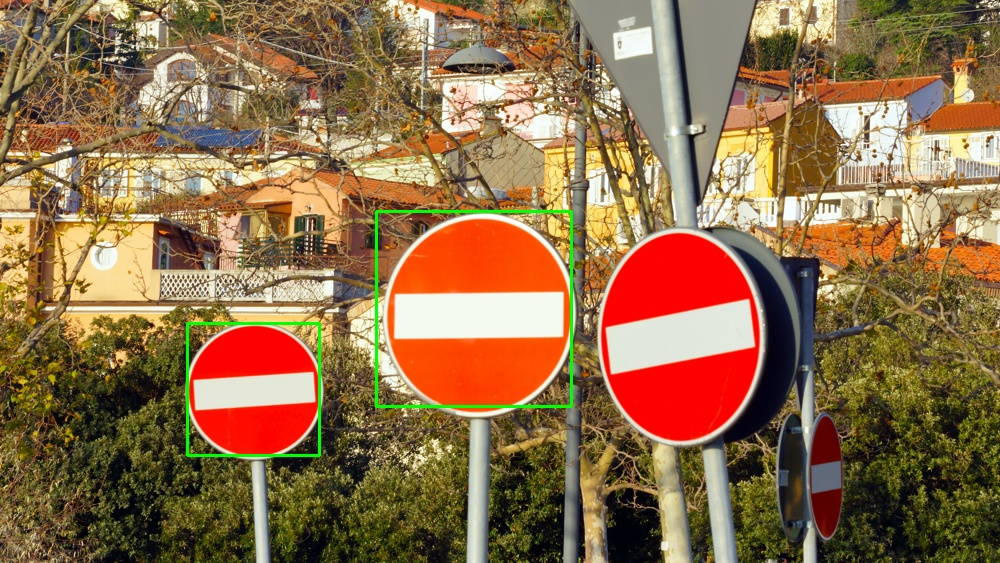
\includegraphics[width = 0.24\textwidth]{images/task_4_6.jpg}\label{fig:improved_image_6}}
  \hfill
  \subfloat[\texttt{NoEntry13.jpg} with detected bounding boxes]{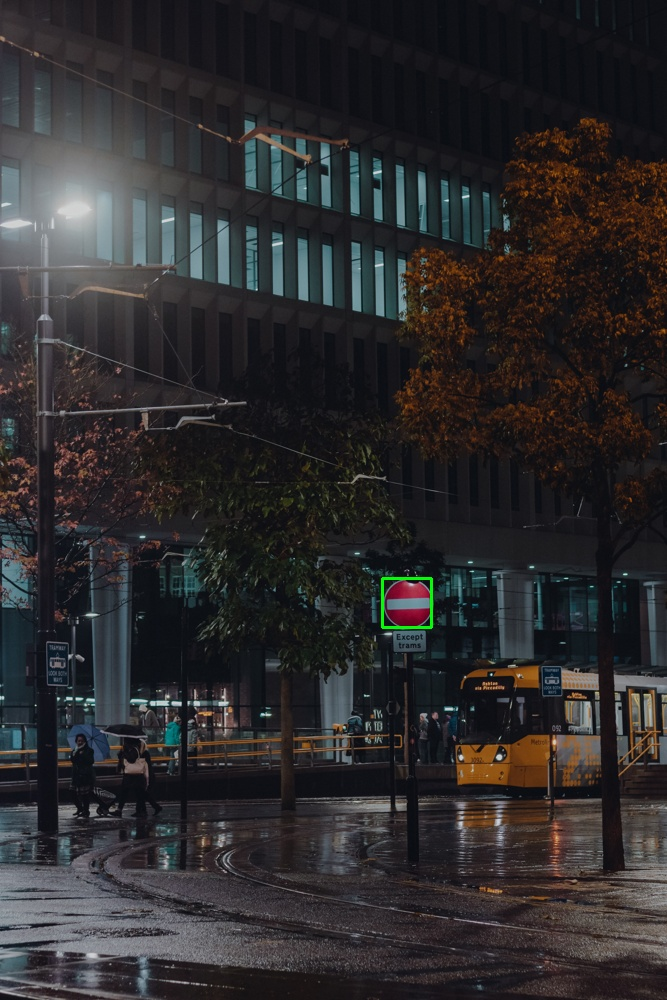
\includegraphics[width = 0.24\textwidth]{images/task_4_13.jpg}\label{fig:improved_image_13}}
  \hfill
  \caption{Two no entry sign images with detected bounding boxes from my improved detector}\label{fig:improved_images}
\end{figure}

Figure \ref{fig:improved_images} exhibits the merit of my improved approach.
All three detected bounding boxes were not identified by the previous detector.

The two bounding boxes in Figure \ref{fig:improved_image_6} very clearly contain no entry signs.
They are detected by the circle Hough transform but not the Viola-Jones detector.
Therefore, my improved algorithm puts them through the extra stage of processing.
First, the pixels are converted from RGB to LAB, and $k$-means is performed with $k = 2$.
This very clearly identifies the two main colours.
The merit of using $k$-means is very evident here: without it, the two main colours would not be able to be identified.
To confirm the two main colours are red and white, the Euclidean distance is computed.
Since they are, the detector looks for two horizontal parallel lines, which it finds, and therefore positively identifies the object as a no entry sign.
The merit of using the line Hough transform is evident here: without it, any circles containing primary red and white would be a false positive.

The no entry sign in Figure \ref{fig:improved_image_13} is clearly a no entry sign, but potentially due to the very low lighting it is not identified by the Viola-Jones detector.
However, it is detected by the circle Hough transform and is therefore put through the extra stage of processing.
Since I converted the colour space of the image to LAB, by focusing on the $a*$ and $b*$ axes and not the $L*$ perceptual brightness axis, my improved detector was still able to identify that the main colours in the circle were red and white.
The merit of converting the colour space from RGB to LAB is evident here: by focusing purely on the $a*$ and $b*$ axes, no entry signs are able to be identified even in bad lighting conditions.
By further confirming it contained two horizontal parallel lines, my detector was able to identify it as a no entry sign.

\subsection{Evaluate}

\begin{table}[htbp]
  \begin{center}
  \caption{TPRs and F\textsubscript{1} scores of the improved implementation and the differences compared to the previous implementation}\label{tab:final}
  \begin{tabular}{l | l l | l l} 
    \hline\hline
    &\multicolumn{2}{| c |}{Result}&\multicolumn{2}{| c}{Difference}\\
    Image&TPR&F\textsubscript{1} Score&TPR&F\textsubscript{1} Score\\
    \hline
    \texttt{NoEntry0.jpg}&1.00&1.00&$\pm0.00$&$\pm0.00$\\
    \texttt{NoEntry1.jpg}&1.00&1.00&$\pm0.00$&$\pm0.00$\\
    \texttt{NoEntry2.jpg}&1.00&1.00&$\pm0.00$&$\pm0.00$\\
    \texttt{NoEntry3.jpg}&1.00&1.00&$\pm0.00$&$\pm0.00$\\
    \texttt{NoEntry4.jpg}&1.00&1.00&$\pm0.00$&$\pm0.00$\\
    \texttt{NoEntry5.jpg}&0.20&0.31&$\pm0.00$&$\pm0.00$\\
    \texttt{NoEntry6.jpg}&0.50&0.67&+0.50&+0.67\\
    \texttt{NoEntry7.jpg}&0.00&0.00&$\pm0.00$&$\pm0.00$\\
    \texttt{NoEntry8.jpg}&0.43&0.60&$\pm0.00$&$\pm0.00$\\
    \texttt{NoEntry9.jpg}&1.00&1.00&$\pm0.00$&$\pm0.00$\\
    \texttt{NoEntry10.jpg}&1.00&1.00&$\pm0.00$&$\pm0.00$\\
    \texttt{NoEntry11.jpg}&1.00&1.00&+0.50&+0.33\\
    \texttt{NoEntry12.jpg}&0.38&0.55&$\pm0.00$&$\pm0.00$\\
    \texttt{NoEntry13.jpg}&1.00&1.00&+1.00&+1.00\\
    \texttt{NoEntry14.jpg}&1.00&1.00&$\pm0.00$&$\pm0.00$\\
    \texttt{NoEntry15.jpg}&1.00&1.00&$\pm0.00$&$\pm0.00$\\
    \hdashline
    All images&0.58&0.73&+0.08&+0.07\\
    \hline
  \end{tabular}
  \end{center}
\end{table}

Table \ref{tab:final} contains the TPR and F\textsubscript{1} scores of the improved detector.
By putting detected circles that were not detected by the Viola-Jones detector through an extra stage or processing, the improved implementation was able to detect 8\% more no entry signs, and achieved a 7\% higher F\textsubscript{1} score.
The key merits and shortcomings of the improved implementation include:
\begin{itemize}
  \item No entry signs that are facing the camera (i.e. circles) are identified almost always by the circle Hough transform, and by putting them through the extra stage of processing they are almost always correctly identified by looking for key characteristics
  \item No entry signs that are not detected by the circle Hough transform cannot be detected no matter what; this includes no entry signs that are at an angle (and are therefore an ellipse) and no entry signs with a significant amount of occlusion
\end{itemize}

\clearpage

\onecolumn{\printbibliography}
    

\end{document}